\documentclass{standalone}
\usepackage{tikz,ctex}
\usepackage{tikz-3dplot} % 2-1
\usepackage{unicode-math} % 2-5,4-1,4-2
\setmathfont{Fira Math Regular}
\setmainfont{Fira Sans}
\definecolor{background}{RGB}{239, 239, 239} % 4-5,6-2,6-5
\begin{document}
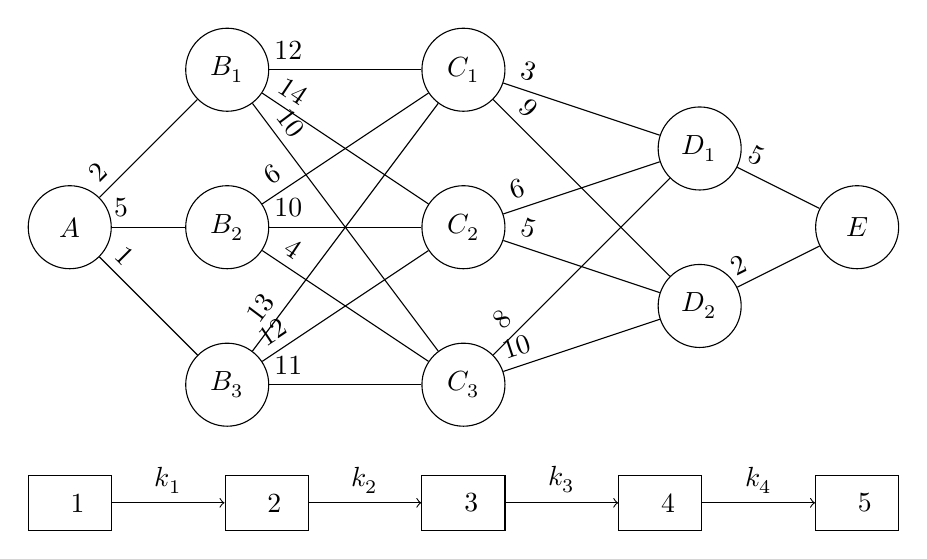
\begin{tikzpicture}
\foreach \x/\y/\text[count=\i] in{0/0/A,2/2/B_1,2/0/B_2,2/-2/B_3,5/2/C_1,5/0/C_2,5/-2/C_3,8/1/D_1,8/-1/D_2,10/0/E}{
    \node[circle,minimum width=30pt,draw] (\i) at(\x,\y){$\text$};}
\foreach \u/\v/\num in{1/2/2,1/3/5,1/4/1,2/5/12,2/6/14,2/7/10,3/5/6,3/6/10,3/7/4,4/5/13,4/6/12,4/7/11,5/8/3,5/9/9,6/8/6,6/9/5,7/8/8,7/9/10,8/10/5,9/10/2}{
    \draw (\u) --(\v) node[very near start,sloped,above]{\num};}
\foreach \i in{1,...,5}{
    \node[rectangle,minimum width=30pt,minimum height=20pt, draw] (\i) at(2.5*\i-2.5,-3.5) {状态\i};}
\foreach \v[count=\u] in{2,...,5}{
    \draw[->] (\u)--(\v) node[midway,above]{$k_\u$};}
\end{tikzpicture}
\end{document}